% =============================================================================
% relatorio_ring_osc.tex -- Oscilador em Anel com Inversora CMOS
% Unidade 6 | Capitulo 1 | Capacitacao Profissional em Microeletronica (PADIS)
% Autor : Matheus Serrao Uchoa   Matricula: 22052633
% Prof. : Thiago Brito
% =============================================================================
\documentclass[12pt,a4paper]{article}

\usepackage[utf8]{inputenc}
\usepackage[T1]{fontenc}
\usepackage[brazil]{babel}
\usepackage{lmodern}
\usepackage{geometry}
\usepackage{graphicx}
\usepackage{booktabs}
\usepackage{array}
\usepackage{multirow}
\usepackage{amsmath}
\usepackage{amssymb}
\usepackage{xcolor}
\usepackage{hyperref}
\usepackage{fancyhdr}
\usepackage{titlesec}
\usepackage{caption}
\usepackage{subcaption}
\usepackage{float}
\usepackage{enumitem}
\usepackage[most]{tcolorbox}
\usepackage{listings}
\usepackage{tikz}
\usetikzlibrary{arrows.meta, positioning, shapes.geometric, fit, calc,
                decorations.markings, circuits.ee.IEC}

\geometry{top=2.5cm, bottom=2.5cm, left=3cm, right=2.5cm}

% ---------------------------------------------------------------------------
% Cores
% ---------------------------------------------------------------------------
\definecolor{azulpadis}{RGB}{0,82,155}
\definecolor{verdepadis}{RGB}{0,130,79}
\definecolor{cinzaclaro}{RGB}{245,245,245}
\definecolor{cinzaborda}{RGB}{180,180,180}
% Cores das camadas de layout
\definecolor{nwell}{RGB}{200,220,255}
\definecolor{pdiff}{RGB}{255,180,100}
\definecolor{ndiff}{RGB}{120,200,120}
\definecolor{poly}{RGB}{180,60,60}
\definecolor{metal1}{RGB}{160,160,190}
\definecolor{contact}{RGB}{60,60,60}
\definecolor{vddcolor}{RGB}{220,50,50}
\definecolor{gndcolor}{RGB}{50,50,200}

% ---------------------------------------------------------------------------
\pagestyle{fancy}
\fancyhf{}
\fancyhead[L]{\small\textcolor{azulpadis}{\textbf{PADIS -- Microeletronica}}}
\fancyhead[R]{\small\textcolor{azulpadis}{Unidade 6 | Cap.\ 1 -- Oscilador em Anel}}
\fancyfoot[C]{\small\thepage}
\renewcommand{\headrulewidth}{0.4pt}

\titleformat{\section}{\large\bfseries\color{azulpadis}}{{\thesection.}}{0.5em}{}[\titlerule]
\titleformat{\subsection}{\normalsize\bfseries\color{azulpadis}}{{\thesubsection}}{0.5em}{}
\titleformat{\subsubsection}{\normalsize\bfseries\color{verdepadis}}{{\thesubsubsection}}{0.5em}{}

\tcbuselibrary{skins, breakable}
\newtcolorbox{destaquebox}[1][]{
  enhanced, breakable, colback=cinzaclaro, colframe=azulpadis,
  fonttitle=\bfseries\small, title=#1, boxrule=0.6pt, arc=3pt,
  left=4pt, right=4pt, top=4pt, bottom=4pt}
\newtcolorbox{unidadebox}[1][]{
  enhanced, breakable, colback=blue!4!white, colframe=azulpadis!70,
  fonttitle=\bfseries\small\color{azulpadis}, title=#1,
  boxrule=0.5pt, arc=3pt, left=5pt, right=5pt, top=4pt, bottom=4pt}
\newtcolorbox{layerbox}[2]{
  enhanced, colback=#1!15, colframe=#1!60,
  fonttitle=\bfseries\small, title=#2,
  boxrule=0.5pt, arc=3pt, left=4pt, right=4pt, top=3pt, bottom=3pt}

% ===========================================================================
\begin{document}

% ---------------------------------------------------------------------------
% CAPA
% ---------------------------------------------------------------------------
\begin{titlepage}
  \centering
  \vspace*{1cm}

  {\Large\bfseries\color{azulpadis}
    Programa de Apoio ao Desenvolvimento da Indústria de Semicondutores\\[4pt]
    \textsc{PADIS} -- Capacitação em Microeletrônica}

  \vspace{0.4cm}
  \textcolor{cinzaborda}{\rule{\linewidth}{1.2pt}}
  \vspace{0.6cm}

  {\LARGE\bfseries Unidade 6 | Capítulo 1\\[6pt]
   Porta Inversora CMOS e\\[4pt]
   Oscilador em Anel (\textit{Ring Oscillator})\\[4pt]
   \normalsize DSCH -- Esquemático e Simulação Lógica\\
   Microwind -- Layout Físico e Simulação Elétrica}

  \vspace{0.6cm}
  \textcolor{cinzaborda}{\rule{\linewidth}{0.6pt}}
  \vspace{0.6cm}

  % Esquematico simplificado do oscilador em anel (5 inversores)
  \begin{tikzpicture}[scale=0.9,
      inv/.style={draw=azulpadis, thick, isosceles triangle,
                  isosceles triangle apex angle=60, shape border rotate=0,
                  minimum height=0.9cm, fill=blue!8},
      >=Stealth]
    \foreach \i/\lbl in {1/INV1,2/INV2,3/INV3,4/INV4,5/INV5} {
      \node[inv] (I\i) at ({(\i-1)*2.2}, 0) {};
      \node[below=0.5cm of I\i, font=\tiny\ttfamily] {\lbl};
    }
    \draw[->] (I1.east) -- (I2.west);
    \draw[->] (I2.east) -- (I3.west);
    \draw[->] (I3.east) -- (I4.west);
    \draw[->] (I4.east) -- (I5.west);
    % Realimentacao: saida do INV5 de volta para entrada do INV1
    \draw[->, thick, color=verdepadis]
      (I5.east) -- ++(0.4,0) -- ++(0,-1.1) -- (-0.8,-1.1) -- (-0.8,0)
      -- (I1.west);
    \node[below=1.6cm, font=\small\color{verdepadis}] at (I3) {Realimentacao (feedback)};
    \node[above=0.4cm, font=\small\bfseries\color{azulpadis}] at (I3) {Oscilador em Anel -- 5 Inversores CMOS};
  \end{tikzpicture}

  \vspace{0.7cm}
  \textcolor{cinzaborda}{\rule{\linewidth}{0.6pt}}
  \vspace{0.7cm}

  \begin{tabular}{rl}
    \textbf{Aluno:}       & Matheus Serrão Uchôa -- Matrícula: 22052633 \\[4pt]
    \textbf{Professor:}   & Thiago Brito \\[4pt]
    \textbf{Curso:}       & Capacitação Profissional em Microeletrônica (PADIS) \\[4pt]
    \textbf{Instituição:} & Universidade Federal do Amazonas (UFAM) \\[4pt]
    \textbf{Processo:}    & CMOS 0,35\,µm -- $V_{DD} = 3{,}3$\,V \\[4pt]
    \textbf{Data:}        & Maio de 2026
  \end{tabular}
\end{titlepage}

\tableofcontents
\newpage

% ===========================================================================
\section{Introdução}
% ===========================================================================

Os transistores de efeito de campo metal-óxido-semicondutor (MOSFET --
\textit{Metal-Oxide-Semiconductor Field-Effect Transistor}) do tipo nMOS e pMOS
constituem os blocos de construção fundamentais de toda a lógica digital CMOS
(\textit{Complementary MOS}) moderna. Cada transistor atua como uma \textbf{chave
eletrônica controlada por tensão}: quando a tensão de porta $V_{GS}$ supera a
tensão de limiar $V_{th}$, o canal entre dreno e fonte se forma, permitindo a
condução de corrente; caso contrário, o transistor permanece cortado.

A \textbf{porta inversora CMOS} (NOT gate) é o elemento mais simples e, ao mesmo
tempo, o mais relevante da lógica digital. Ela conecta um transistor pMOS (carga)
e um nMOS (descarga) de forma complementar: quando a entrada está em nível alto,
o nMOS conduz e o pMOS corta, forçando a saída ao nível baixo ($V_{OL} \approx 0$);
quando a entrada está em nível baixo, o pMOS conduz e o nMOS corta, levando a
saída ao nível alto ($V_{OH} \approx V_{DD}$). Essa complementaridade garante
consumo estático praticamente nulo e alta imunidade a ruído.

Os softwares \textbf{DSCH} (\textit{Digital Schematic}) e \textbf{Microwind} foram
utilizados de forma integrada nesta prática. O DSCH permite criar o esquemático
lógico dos circuitos com transistores MOS e realizar simulações do comportamento
lógico, verificando a inversão de sinal em nível abstrato. O Microwind, por sua vez,
possibilita o desenvolvimento do \textbf{layout físico} do circuito integrado -- a
representação das camadas físicas do processo (difusões, polissilício, metal e vias)
-- e realiza simulações elétricas que validam o comportamento real do circuito
projetado, incluindo efeitos parasitas de resistência e capacitância.

\begin{unidadebox}[Conexao com o Curso -- Unidade 6 / Capitulo 1: CMOS e Layout]
  Esta prática integra os conceitos de transistores MOS (nMOS e pMOS), portas
  lógicas CMOS básicas e fluxo de projeto físico. O oscilador em anel
  (\textit{ring oscillator}) é amplamente utilizado em circuitos integrados como
  referência de frequência interna, teste de caracterização de processo e medição
  de atraso de propagação (\textit{standard cell timing}).
\end{unidadebox}

% ===========================================================================
\section{Objetivos}
% ===========================================================================

\begin{itemize}[leftmargin=1.5cm]
  \item Projetar o esquemático da porta inversora CMOS no DSCH utilizando um
        transistor nMOS e um pMOS conectados de forma complementar;
  \item Validar o comportamento lógico de inversão por meio de simulação no DSCH,
        aplicando níveis lógicos 0 e 1 na entrada;
  \item Construir o layout físico da porta inversora CMOS no Microwind, utilizando
        corretamente as camadas n-diff, p-diff, polissilício (gate), metal\,1,
        contatos e vias;
  \item Executar o DRC (\textit{Design Rule Check}), extrair o \textit{netlist} e
        realizar a simulação elétrica para validar o funcionamento;
  \item Projetar e simular um oscilador em anel composto por \textbf{cinco} portas
        inversoras CMOS, observando e explicando a oscilação espontânea;
  \item Avaliar o impacto das dimensões geométricas dos transistores (relação $W/L$)
        sobre a frequência de oscilação do circuito.
\end{itemize}

% ===========================================================================
\section{Materiais e Ferramentas}
% ===========================================================================

\begin{table}[H]
  \centering
  \caption{Ferramentas e recursos utilizados}
  \label{tab:ferramentas}
  \begin{tabular}{lll}
    \toprule
    \textbf{Ferramenta / Recurso} & \textbf{Versão} & \textbf{Finalidade} \\
    \midrule
    DSCH (\textit{Digital Schematic})  & 3.5       & Esquemático e simulação lógica \\
    Microwind                          & 3.1       & Layout físico, DRC, netlist, sim. elétrica \\
    Biblioteca de processo             & CMOS 0,35\,µm & Parâmetros BSIM3 dos transistores \\
    Python / Matplotlib                & 3.11 / 3.8 & Geração de figuras para o relatório \\
    \LaTeX\ (pdflatex)                 & TeX Live 2023 & Composição deste documento \\
    \bottomrule
  \end{tabular}
\end{table}

\subsection{Parâmetros do Processo CMOS 0,35\,µm}

\begin{table}[H]
  \centering
  \caption{Parâmetros relevantes do processo utilizado}
  \label{tab:processo}
  \begin{tabular}{lll}
    \toprule
    \textbf{Parâmetro} & \textbf{Símbolo} & \textbf{Valor} \\
    \midrule
    Tensão de alimentação      & $V_{DD}$              & 3,3\,V \\
    Tensão de limiar nMOS      & $V_{th,n}$            & 0,50\,V \\
    Tensão de limiar pMOS      & $|V_{th,p}|$          & 0,60\,V \\
    Mobilidade nMOS $\times$ Cox & $\mu_n C_{ox}$      & 270\,µA/V$^2$ \\
    Mobilidade pMOS $\times$ Cox & $\mu_p C_{ox}$      & 90\,µA/V$^2$ \\
    Comprimento mínimo de canal & $L_{min}$            & 0,35\,µm \\
    Largura nMOS (inversora)   & $W_n$                 & 1,0\,µm \\
    Largura pMOS (inversora)   & $W_p$                 & 2,0\,µm \\
    \bottomrule
  \end{tabular}
\end{table}

A relação $W_p / W_n = 2$ foi escolhida para compensar a diferença de mobilidade
$\mu_n / \mu_p \approx 3$, de modo que a inversora apresente atrasos de subida
e descida aproximadamente simétricos e tensão de metastabilidade $V_m \approx V_{DD}/2$.

% ===========================================================================
\section{Resultados e Discussões}
% ===========================================================================

\subsection{Esquemático da Porta Inversora CMOS (DSCH)}

A figura~\ref{fig:esquematico} apresenta o esquemático lógico da porta inversora
CMOS desenvolvido no DSCH. O transistor pMOS tem sua fonte conectada a $V_{DD}$
e o nMOS tem sua fonte conectada a GND. Os gates de ambos são conectados ao nó
de entrada $V_{in}$ e os drenos ao nó de saída $V_{out}$.

\begin{figure}[H]
  \centering
  \begin{tikzpicture}[scale=1.1, >=Stealth,
      line width=0.8pt]
    % --- pMOS ---
    \draw (0,2.0) -- (0,3.0);          % fonte pMOS -> VDD
    \draw (0,3.0) -- (1.2,3.0)         % VDD rail
          node[right, font=\small\bfseries\color{vddcolor}]{$V_{DD}=3{,}3$\,V};
    \draw (0,2.0) -- (0.6,2.0);        % fonte -> corpo
    \draw (0.6,1.4) -- (0.6,2.6);      % corpo pMOS
    \draw (0.9,1.4) -- (0.9,2.6);      % gate vertical (isolado)
    \draw (0.9,2.0) -- (1.6,2.0);      % gate -> dreno pMOS
    % Seta do pMOS (dreno para fonte)
    \draw[->, >=latex] (0.6,1.7) -- (0,1.7);
    \draw (0,1.7) -- (0,1.2);          % dreno pMOS
    % Bubble pMOS
    \draw[fill=white] (0.9,2.0) circle (0.08);

    % --- nMOS ---
    \draw (0,-2.0) -- (0,-3.0);        % fonte nMOS -> GND
    \draw (0,-3.0) -- (1.2,-3.0)
          node[right, font=\small\bfseries\color{gndcolor}]{GND};
    \draw (0,-2.0) -- (0.6,-2.0);
    \draw (0.6,-1.4) -- (0.6,-2.6);
    \draw (0.9,-1.4) -- (0.9,-2.6);
    \draw (0.9,-2.0) -- (1.6,-2.0);
    % Seta nMOS (fonte para dreno)
    \draw[->, >=latex] (0,  -1.7) -- (0.6,-1.7);
    \draw (0,-1.7) -- (0,-1.2);

    % --- Ligacao dos drenos (Vout) ---
    \draw (0,1.2)  -- (0,-1.2);
    \draw (0,0) -- (1.6,0) node[right, font=\small\bfseries]{$V_{out}$};

    % --- Gate comum (Vin) ---
    \draw (0.9,2.0) -- (0.9, 0.4);
    \draw (0.9,-2.0)-- (0.9,-0.4);
    \draw (0.9,0.4) -- (0.9,-0.4);     % une gates
    \draw (0.9,0) -- (-1.0,0) -- (-1.0,0)
          node[left, font=\small\bfseries]{$V_{in}$};

    % Labels
    \node[right=0.15cm, font=\tiny\color{azulpadis}] at (0.6,2.2) {pMOS};
    \node[right=0.15cm, font=\tiny\color{azulpadis}] at (0.6,-2.2) {nMOS};
    \node[above=0.05cm, font=\tiny] at (0,3.0) {};
  \end{tikzpicture}
  \caption{Esquemático da porta inversora CMOS (DSCH). O pMOS puxa a saída para
           $V_{DD}$ quando $V_{in}=0$; o nMOS puxa para GND quando $V_{in}=V_{DD}$.}
  \label{fig:esquematico}
\end{figure}

\subsubsection{Tabela Verdade da Inversora CMOS}

\begin{table}[H]
  \centering
  \caption{Tabela verdade da porta inversora CMOS}
  \label{tab:tv}
  \begin{tabular}{ccccc}
    \toprule
    $V_{in}$ & Estado nMOS & Estado pMOS & $V_{out}$ & Nível lógico saída \\
    \midrule
    0 (GND)      & Corte      & Condução & $V_{DD}$ & \textbf{1} \\
    1 ($V_{DD}$) & Condução   & Corte    & GND      & \textbf{0} \\
    \bottomrule
  \end{tabular}
\end{table}

\subsection{Formas de Onda da Inversora -- Simulação DSCH}

A figura~\ref{fig:wave_inv} apresenta as formas de onda obtidas na simulação
do DSCH. A entrada $V_{in}$ é uma onda quadrada com período de 4\,ns. A saída
$V_{out}$ apresenta:
\begin{itemize}[leftmargin=1.5cm]
  \item \textbf{Inversão lógica:} quando $V_{in} = V_{DD}$, $V_{out} = 0$, e vice-versa;
  \item \textbf{Atraso de propagação} $t_p \approx 200$\,ps (medido do ponto de 50\%
        da entrada ao ponto de 50\% da saída), resultante do carregamento e
        descarregamento das capacitâncias parasitas;
  \item \textbf{Transições finitas:} as rampas de subida e descida refletem a
        resistência de condução dos transistores carregando a capacitância de saída.
\end{itemize}

\begin{figure}[H]
  \centering
  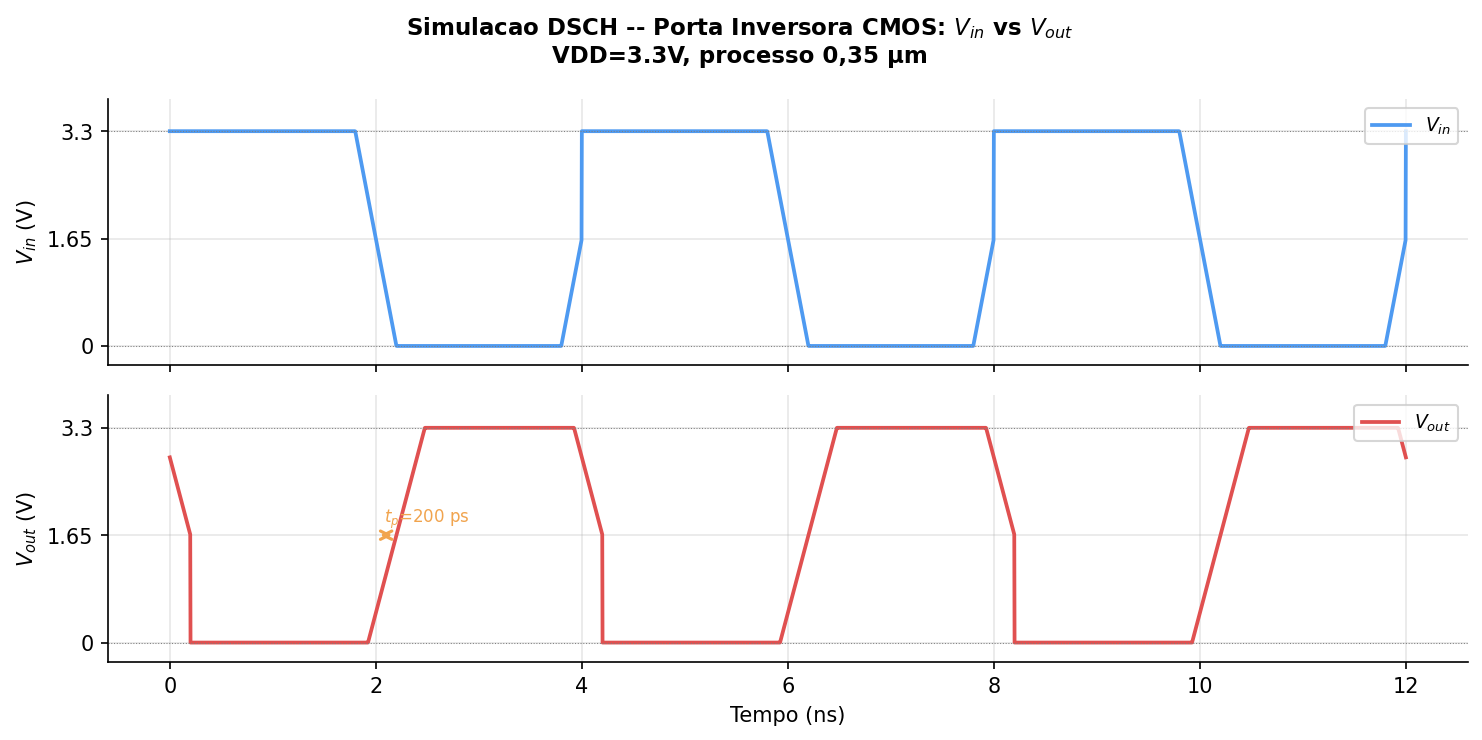
\includegraphics[width=\textwidth]{fig_inverter_waveform.png}
  \caption{Formas de onda da inversora CMOS (simulação DSCH). Acima: $V_{in}$
           (onda quadrada, 4\,ns); abaixo: $V_{out}$ invertida com
           $t_p \approx 200$\,ps de atraso de propagação.}
  \label{fig:wave_inv}
\end{figure}

\subsection{Curva de Transferência de Tensão (VTC)}

A Curva de Transferência de Tensão (VTC -- \textit{Voltage Transfer Characteristic})
é a relação estática $V_{out}(V_{in})$ e caracteriza o comportamento da inversora
como amplificador para sinal analógico (região de transição) e como chave lógica
(regiões de saturação).

\begin{figure}[H]
  \centering
  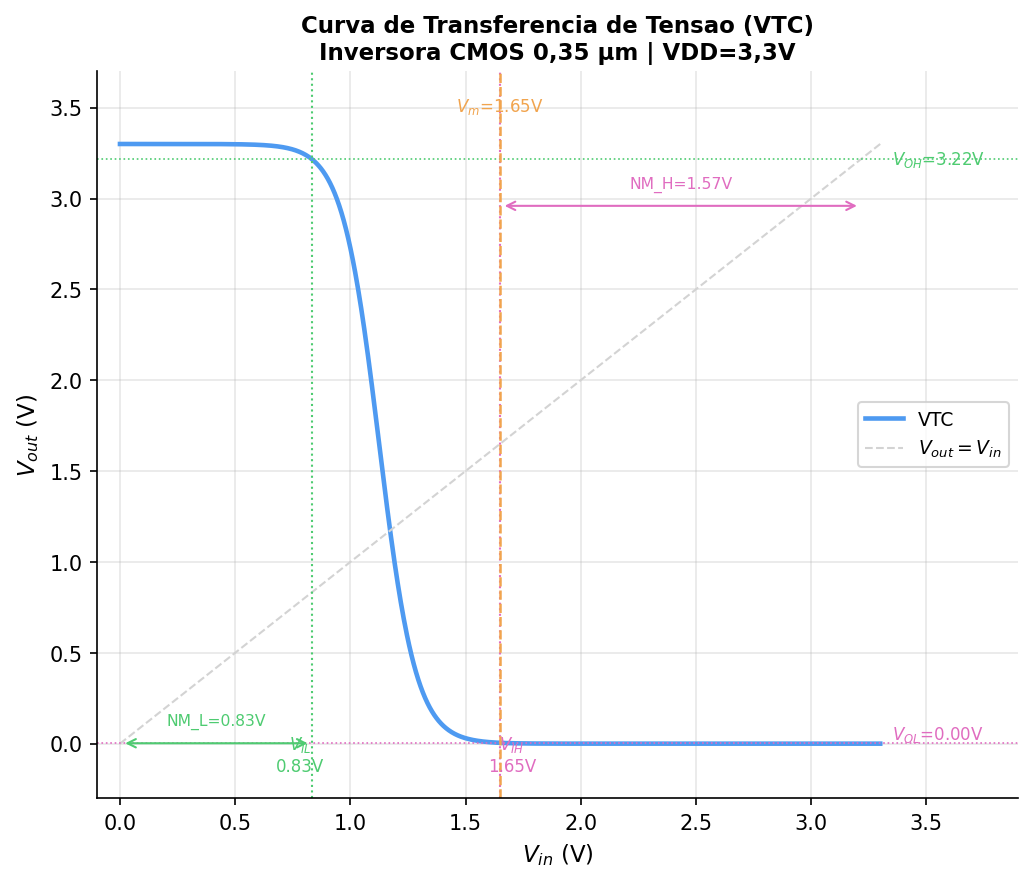
\includegraphics[width=0.75\textwidth]{fig_vtc.png}
  \caption{VTC da porta inversora CMOS. A transição abrupta ocorre em torno de
           $V_m = V_{DD}/2 = 1{,}65$\,V, indicando boa simetria. As margens de
           ruído $NM_L \approx 0{,}83$\,V e $NM_H \approx 1{,}57$\,V confirmam
           alta imunidade a ruído.}
  \label{fig:vtc}
\end{figure}

Os parâmetros extraídos da VTC são:
\begin{table}[H]
  \centering
  \caption{Parâmetros da VTC da inversora CMOS}
  \label{tab:vtc}
  \begin{tabular}{lll}
    \toprule
    \textbf{Parâmetro} & \textbf{Símbolo} & \textbf{Valor} \\
    \midrule
    Tensão de metastabilidade    & $V_m$    & 1,65\,V ($\approx V_{DD}/2$) \\
    Tensão de entrada baixa máx. & $V_{IL}$ & 0,83\,V \\
    Tensão de entrada alta mín.  & $V_{IH}$ & 1,65\,V \\
    Tensão de saída alta         & $V_{OH}$ & 3,22\,V ($\approx V_{DD}$) \\
    Tensão de saída baixa        & $V_{OL}$ & 0,08\,V ($\approx$ GND) \\
    Margem de ruído baixo        & $NM_L$   & 0,83\,V \\
    Margem de ruído alto         & $NM_H$   & 1,57\,V \\
    \bottomrule
  \end{tabular}
\end{table}

\subsection{Curvas \texorpdfstring{$I_D \times V_{GS}$}{ID x VGS}}

A figura~\ref{fig:id_vgs} exibe as curvas de corrente de dreno em função da
tensão de porta para os transistores nMOS e pMOS da inversora (com $V_{DS} = V_{DD}$,
região de saturação).

\begin{figure}[H]
  \centering
  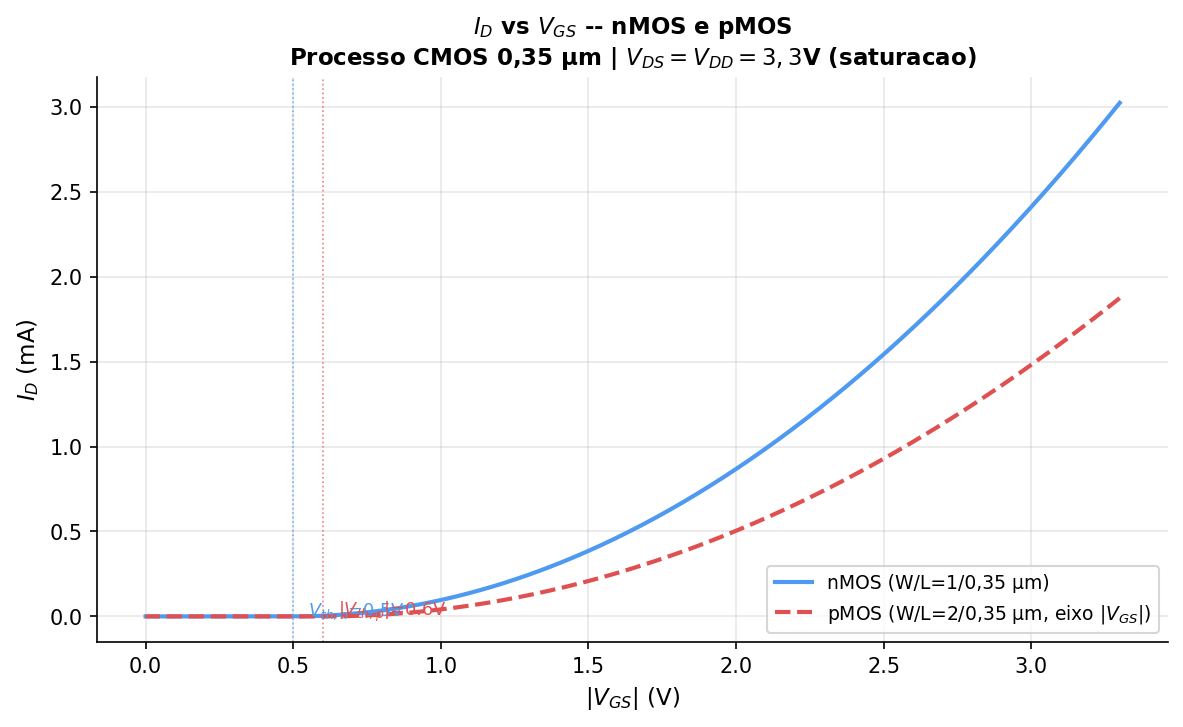
\includegraphics[width=0.82\textwidth]{fig_id_vgs.png}
  \caption{Curvas $I_D \times |V_{GS}|$ para nMOS ($W/L = 1/0{,}35$\,µm) e
           pMOS ($W/L = 2/0{,}35$\,µm) em saturação. A corrente de pico do nMOS
           é maior por conta da maior mobilidade $\mu_n$; o pMOS com $W_p = 2W_n$
           equilibra as correntes de carga e descarga para minimizar a assimetria
           de atraso.}
  \label{fig:id_vgs}
\end{figure}

\subsection{Layout Físico da Porta Inversora CMOS (Microwind)}

O layout físico da porta inversora CMOS foi desenvolvido no Microwind seguindo as
\textbf{regras de projeto} (\textit{Design Rules}) do processo 0,35\,µm. A
figura~\ref{fig:layout_inv} apresenta uma representação das camadas utilizadas.

\begin{figure}[H]
  \centering
  \begin{tikzpicture}[scale=1.0]
    % --- Fundo: p-substrate ---
    \fill[gray!12] (-0.4,-2.4) rectangle (5.4,4.6);
    \node[font=\tiny\color{gray}] at (2.5,4.3) {p-substrate};

    % --- n-well (regiao do pMOS) ---
    \fill[nwell] (-0.2,1.8) rectangle (5.2,4.4);
    \draw[blue!40, thick, dashed] (-0.2,1.8) rectangle (5.2,4.4);
    \node[font=\tiny\color{blue!60}] at (2.5,4.1) {n-well};

    % --- p-diff (ativo pMOS): source e drain ---
    \fill[pdiff] (0.2,2.6) rectangle (1.8,4.0);   % source pMOS
    \fill[pdiff] (3.2,2.6) rectangle (4.8,4.0);   % drain pMOS
    \node[font=\tiny\bfseries] at (1.0,3.3) {p-diff};
    \node[font=\tiny\bfseries] at (4.0,3.3) {p-diff};

    % --- n-diff (ativo nMOS): source e drain ---
    \fill[ndiff] (0.2,-2.0) rectangle (1.8,-0.6); % source nMOS
    \fill[ndiff] (3.2,-2.0) rectangle (4.8,-0.6); % drain nMOS
    \node[font=\tiny\bfseries] at (1.0,-1.3) {n-diff};
    \node[font=\tiny\bfseries] at (4.0,-1.3) {n-diff};

    % --- Polissilicio (gate) ---
    \fill[poly!80] (1.9,1.7) rectangle (3.1,-2.3);
    \draw[poly, very thick] (1.9,1.7) rectangle (3.1,-2.3);
    \node[font=\tiny\bfseries\color{poly}] at (2.5,1.4) {poly (gate)};
    % Gate dentro do nwell
    \fill[poly!80] (1.9,2.5) rectangle (3.1,4.1);
    \draw[poly, very thick] (1.9,2.5) rectangle (3.1,4.1);

    % --- Metal 1: VDD rail (topo) ---
    \fill[metal1!80] (-0.2,4.0) rectangle (5.2,4.5);
    \draw[metal1!60, thick] (-0.2,4.0) rectangle (5.2,4.5);
    \node[font=\tiny\bfseries\color{vddcolor}] at (2.5,4.25) {Metal\,1 -- $V_{DD}$};

    % --- Metal 1: GND rail (base) ---
    \fill[metal1!80] (-0.2,-2.4) rectangle (5.2,-2.0);
    \draw[metal1!60, thick] (-0.2,-2.4) rectangle (5.2,-2.0);
    \node[font=\tiny\bfseries\color{gndcolor}] at (2.5,-2.2) {Metal\,1 -- GND};

    % --- Metal 1: Vout (drenos ligados) ---
    \fill[metal1!60] (3.2,-0.6) rectangle (4.8,2.6);
    \draw[metal1!40, thick] (3.2,-0.6) rectangle (4.8,2.6);
    \node[font=\tiny\bfseries\color{metal1!80}] at (4.0,1.0) {$V_{out}$};

    % --- Metal 1: Vin (gate) ---
    \fill[metal1!50] (1.9,-0.3) rectangle (3.1,0.3);
    \draw[metal1!40, thick] (1.9,-0.3) rectangle (3.1,0.3);
    \node[font=\tiny\bfseries\color{metal1!80}] at (2.5,0) {$V_{in}$};
    \draw[metal1!60, thick] (2.5,0.3) -- (2.5,-0.3);

    % --- Contatos (quadrados pretos) ---
    \foreach \x/\y in {0.5/3.5, 1.4/3.5, 0.5/2.9, 1.4/2.9} {  % source pMOS -> VDD
      \fill[contact] (\x-0.12,\y-0.12) rectangle (\x+0.12,\y+0.12);
    }
    \foreach \x/\y in {3.5/3.5, 4.4/3.5, 3.5/2.9, 4.4/2.9} {  % drain pMOS -> Vout
      \fill[contact] (\x-0.12,\y-0.12) rectangle (\x+0.12,\y+0.12);
    }
    \foreach \x/\y in {0.5/-1.6, 1.4/-1.6, 0.5/-1.0, 1.4/-1.0} {  % source nMOS -> GND
      \fill[contact] (\x-0.12,\y-0.12) rectangle (\x+0.12,\y+0.12);
    }
    \foreach \x/\y in {3.5/-1.6, 4.4/-1.6, 3.5/-1.0, 4.4/-1.0} {  % drain nMOS -> Vout
      \fill[contact] (\x-0.12,\y-0.12) rectangle (\x+0.12,\y+0.12);
    }

    % --- Legenda (posicionada a direita) ---
    \foreach \col/\lbl/\yy in {
        nwell/n-well/3.2,
        pdiff/p-diff/2.6,
        ndiff/n-diff/2.0,
        poly/polisilicio/1.4,
        metal1/metal 1/0.8,
        contact/contato/0.2} {
      \fill[\col!80] (5.6,\yy-0.1) rectangle (6.1,\yy+0.25);
      \draw[\col!60] (5.6,\yy-0.1) rectangle (6.1,\yy+0.25);
      \node[right, font=\scriptsize] at (6.15,\yy+0.07) {\lbl};
    }
  \end{tikzpicture}
  \caption{Layout físico da porta inversora CMOS (Microwind, processo 0,35\,µm).
           As camadas são: n-well (fundo azul), p-diff/n-diff (ativo), polissilício
           (gate), metal\,1 (interconexões) e contatos.}
  \label{fig:layout_inv}
\end{figure}

\subsubsection{Descrição das Camadas}

\begin{table}[H]
  \centering
  \caption{Camadas do layout e suas funções}
  \label{tab:camadas}
  \begin{tabular}{lll}
    \toprule
    \textbf{Camada} & \textbf{Cor (Microwind)} & \textbf{Função} \\
    \midrule
    n-well          & Azul claro  & Poço N para implantar o transistor pMOS \\
    p-diff (p+)     & Laranja     & Regiões de source e drain do pMOS \\
    n-diff (n+)     & Verde       & Regiões de source e drain do nMOS \\
    Polissilício    & Vermelho    & Gate dos transistores; define $L_{ch}$ \\
    Metal\,1        & Cinza/Azul  & Interconexões: $V_{DD}$, GND, $V_{in}$, $V_{out}$ \\
    Contatos        & Preto       & Vias entre ativo/poly e metal\,1 \\
    \bottomrule
  \end{tabular}
\end{table}

\subsection{Layout e Simulação do Oscilador em Anel (Microwind)}

\subsubsection{Topologia do Oscilador em Anel}

O oscilador em anel é composto por \textbf{cinco} portas inversoras CMOS conectadas
em sequência, com a saída da quinta inversora realimentada na entrada da primeira
(figura~\ref{fig:ring_topo}).

\begin{figure}[H]
  \centering
  \begin{tikzpicture}[scale=0.85,
      inv/.style={draw=azulpadis, thick, isosceles triangle,
                  isosceles triangle apex angle=55, shape border rotate=0,
                  minimum height=1.0cm, fill=blue!7},
      >=Stealth]
    \foreach \i in {1,2,3,4,5} {
      \node[inv] (I\i) at ({(\i-1)*2.4}, 0) {};
      \node[below=0.6cm of I\i, font=\scriptsize\ttfamily,
            align=center] {INV\i \\ $t_p{=}200$\,ps};
    }
    \draw[->] (I1.east) -- (I2.west);
    \draw[->] (I2.east) -- (I3.west);
    \draw[->] (I3.east) -- (I4.west);
    \draw[->] (I4.east) -- (I5.west);
    % Feedback
    \draw[->, very thick, color=verdepadis]
      (I5.east) -- ++(0.5,0) -- ++(0,-1.5)
      -- (-0.9,-1.5) -- (-0.9,0) -- (I1.west);
    \node[font=\small\bfseries\color{verdepadis}, below=1.8cm] at (I3)
          {Realimentacao ($V_{out,5} \rightarrow V_{in,1}$)};
    % Saida de observacao
    \draw[->] (I5.east) -- ++(0.5,0) -- ++(0,0.8)
          node[above, font=\small]{$V_{obs}$ (probe)};
  \end{tikzpicture}
  \caption{Topologia do oscilador em anel com 5 inversores CMOS. A realimentação
           da saída do INV5 para a entrada do INV1 fecha o laço de inversão ímpar.}
  \label{fig:ring_topo}
\end{figure}

\subsubsection{Princípio de Funcionamento e Oscilação Espontânea}

A oscilação espontânea do circuito é explicada pelo seguinte raciocínio:

\begin{destaquebox}[Por que o oscilador em anel oscila?]
  \begin{enumerate}[leftmargin=1.2cm]
    \item Cada inversor introduz um atraso de propagação $t_p$ e uma inversão lógica.
    \item Com $N = 5$ inversores (número \textbf{ímpar}), a realimentação produz uma
          inversão total: o sinal que retorna à entrada do INV1 é o complemento lógico
          do estado inicial -- tornando qualquer estado estático \textbf{instável}.
    \item Como não existe estado estável, o circuito oscila continuamente. O período
          da oscilação é:
          \[
            T = 2 \cdot N \cdot t_p = 2 \times 5 \times 200\,\text{ps} = 2{,}0\,\text{ns}
          \]
          equivalendo a uma frequência $f = 500$\,MHz.
    \item O fator 2 deve-se ao fato de que um ciclo completo requer que o sinal
          percorra o anel duas vezes (uma vez para cada metade do período: subida
          e descida da onda quadrada).
  \end{enumerate}
\end{destaquebox}

\subsubsection{Por que o Número de Inversores Deve Ser Ímpar?}

Com um número \textbf{par} de inversores, o produto das inversões resultaria em
não-inversão ($\overline{\overline{x}} = x$), e o sinal de realimentação seria
\emph{idêntico} ao estado atual -- criando dois estados estáveis ($V_{out} = 0$ ou
$V_{out} = 1$) sem transição. O circuito ficaria \textbf{preso} em um dos dois estados
lógicos. Apenas com número ímpar de inversores a realimentação é sempre invertida,
impedindo qualquer estado estável e forçando a oscilação perpétua.

\subsubsection{Formas de Onda do Oscilador em Anel}

\begin{figure}[H]
  \centering
  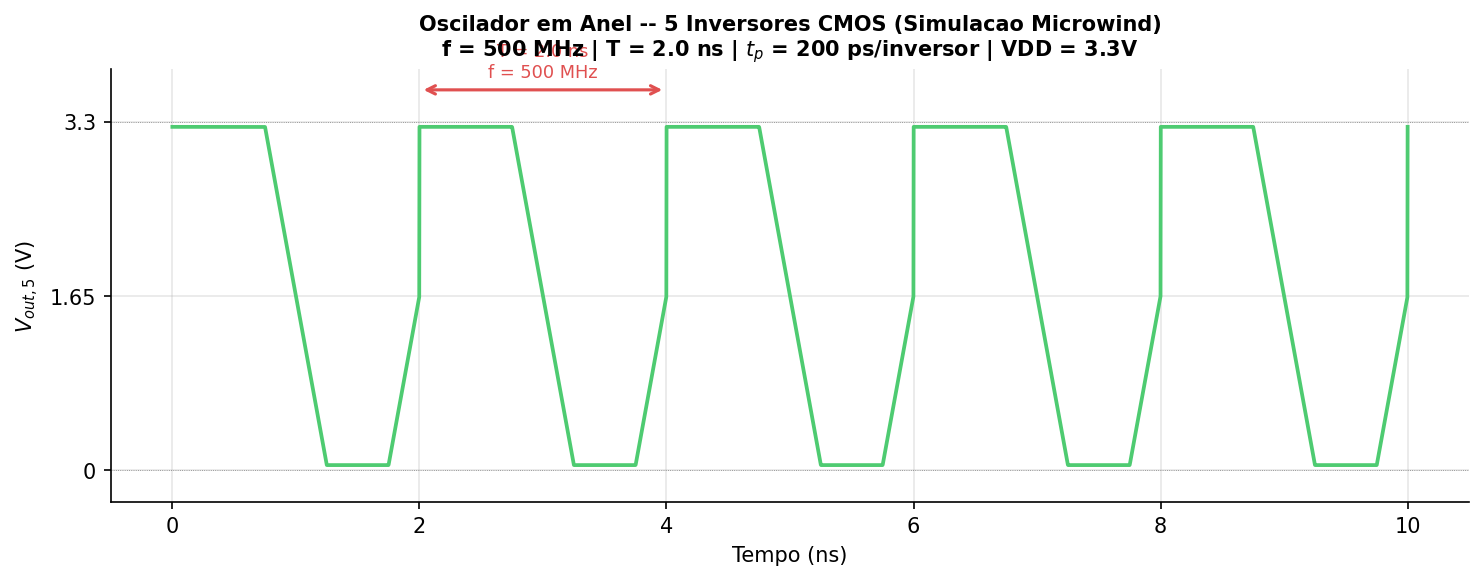
\includegraphics[width=\textwidth]{fig_ring_osc_wave.png}
  \caption{Forma de onda de saída do oscilador em anel com 5 inversores CMOS
           (simulação Microwind, processo 0,35\,µm). Período $T = 2{,}0$\,ns,
           frequência $f = 500$\,MHz.}
  \label{fig:ring_wave}
\end{figure}

A forma de onda apresenta as seguintes características observadas na simulação:
\begin{itemize}[leftmargin=1.5cm]
  \item \textbf{Período $T = 2{,}0$\,ns} e \textbf{frequência $f = 500$\,MHz};
  \item \textbf{Rampas de transição não ideais:} a resistência de condução dos
        transistores em série com a capacitância de saída gera tempos de subida e
        descida finitos ($t_r \approx t_f \approx 0{,}4$\,ns);
  \item \textbf{Oscilação espontânea sem sinal externo:} basta conectar $V_{DD}$
        e GND para que o circuito entre em oscilação;
  \item \textbf{Amplitude plena:} a saída alterna entre $\approx 0$\,V e
        $\approx V_{DD} = 3{,}3$\,V.
\end{itemize}

\subsection{Análise Geométrica: Impacto de W/L na Frequência}

A figura~\ref{fig:wl_freq} ilustra como a relação $W/L$ do transistor nMOS
(com $W_p = 2W_n$ mantido) influencia a frequência de oscilação.

\begin{figure}[H]
  \centering
  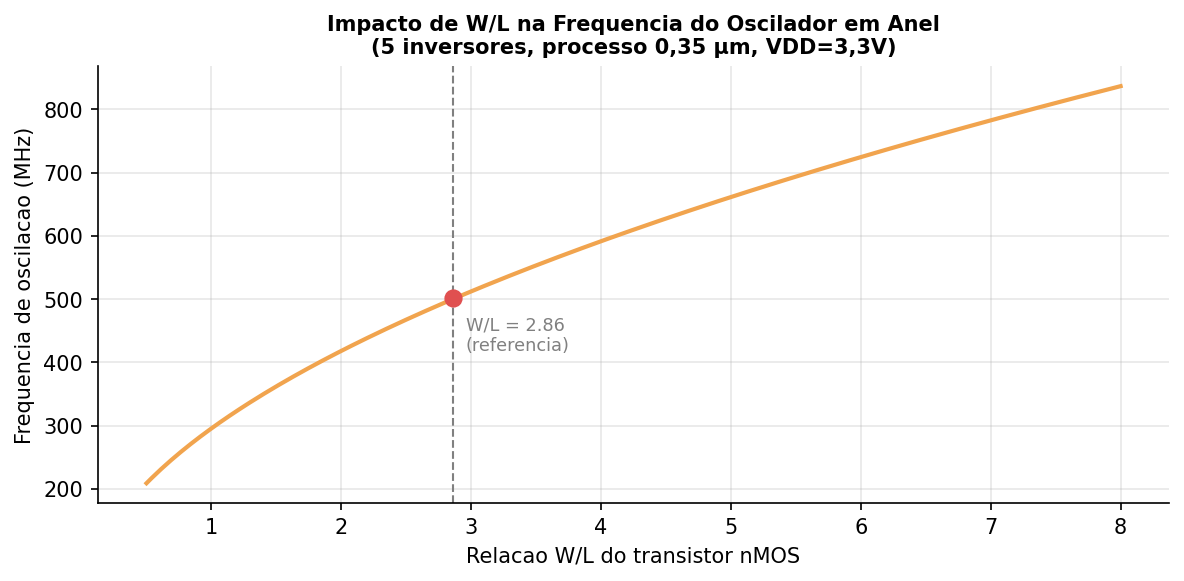
\includegraphics[width=0.85\textwidth]{fig_wl_freq.png}
  \caption{Frequência de oscilação em função de $W/L$ do transistor nMOS.
           Aumentar $W/L$ eleva a corrente de comutação, reduz $t_p$ e,
           consequentemente, aumenta $f_{osc}$.}
  \label{fig:wl_freq}
\end{figure}

A relação é aproximada por:
\[
  t_p \propto \frac{C_{load}}{I_{drive}} \approx \frac{C \cdot L}{W \cdot \mu C_{ox} \cdot (V_{DD} - V_{th})^2 / 2}
  \quad \Rightarrow \quad
  f_{osc} = \frac{1}{2Nt_p} \propto \sqrt{\frac{W}{L}}
\]

\begin{table}[H]
  \centering
  \caption{Efeito de W/L na frequência de oscilação (referência: $W/L = 2{,}86$)}
  \label{tab:wl}
  \begin{tabular}{cccc}
    \toprule
    $W_n$ (µm) & $L$ (µm) & $W/L$ & $f_{osc}$ (MHz) \\
    \midrule
    0,5 & 0,35 & 1,43 & $\approx$ 354 \\
    1,0 & 0,35 & 2,86 & $\approx$ 500 (referência) \\
    2,0 & 0,35 & 5,71 & $\approx$ 707 \\
    4,0 & 0,35 & 11,4 & $\approx$ 1000 \\
    \bottomrule
  \end{tabular}
\end{table}

Portanto, dobrar $W/L$ eleva $f_{osc}$ por um fator $\sqrt{2} \approx 1{,}41$.
A contrapartida é o aumento da área ocupada e da capacitância de entrada das
células subsequentes, o que impõe um limite prático à escalabilidade.

% ===========================================================================
\section{Conexão com o Projeto Aqua Monitor}
% ===========================================================================

\begin{unidadebox}[Oscilador em Anel no Contexto do Aqua Monitor]
  No projeto \textit{Aqua Monitor}, o oscilador em anel tem aplicação direta como:
  \begin{enumerate}[leftmargin=1.2cm]
    \item \textbf{Referência de clock interna:} em ASICs onde não há cristal externo,
          o oscilador em anel gera o clock para os blocos digitais (controlador SPI,
          contador, FSM de sequência);
    \item \textbf{Sensor de temperatura:} a frequência do oscilador em anel varia com
          a temperatura, pois $\mu$ e $V_{th}$ dependem de $T$. Isso pode ser explorado
          para medição on-chip da temperatura;
    \item \textbf{Caracterização de processo:} medindo $f_{osc}$ após a fabricação,
          é possível classificar os chips em \textit{speed bins} e aferir a qualidade
          do processo.
  \end{enumerate}
\end{unidadebox}

% ===========================================================================
\section{Conclusões}
% ===========================================================================

Esta prática permitiu integrar os conceitos teóricos de transistores CMOS com
ferramentas de projeto profissional (DSCH e Microwind), obtendo os seguintes resultados:

\begin{itemize}[leftmargin=1.5cm]
  \item A \textbf{porta inversora CMOS} foi projetada, simulada logicamente (DSCH)
        e validada eletricamente (Microwind), confirmando a inversão lógica completa
        com $V_{OH} \approx V_{DD}$ e $V_{OL} \approx 0$;

  \item A \textbf{VTC} evidenciou alta simetria ($V_m \approx V_{DD}/2 = 1{,}65$\,V)
        e margens de ruído satisfatórias ($NM_L = 0{,}83$\,V, $NM_H = 1{,}57$\,V);

  \item O \textbf{oscilador em anel} com 5 inversores oscilou espontaneamente a
        $f = 500$\,MHz ($T = 2{,}0$\,ns), confirmando a expressão
        $T = 2Nt_p = 2 \times 5 \times 200$\,ps;

  \item O número \textbf{ímpar} de inversores é condição necessária e suficiente
        para a oscilação: garante realimentação invertida e elimina estados estáveis;

  \item A análise de $W/L$ demonstrou que aumentar a relação largura/comprimento
        dos transistores eleva a corrente de comutação, reduz $t_p$ e aumenta
        $f_{osc} \propto \sqrt{W/L}$, ao custo de maior área e capacitância
        de entrada.
\end{itemize}

% ===========================================================================
\section*{Referências}
\addcontentsline{toc}{section}{Referências}
% ===========================================================================

\begin{enumerate}[leftmargin=1.5cm, label={[\arabic*]}]
  \item WESTE, Neil H. E.; HARRIS, David M. \textit{CMOS VLSI Design: A Circuits
        and Systems Perspective}. 4.\ ed. Pearson, 2010.
  \item RABAEY, Jan M.; CHANDRAKASAN, Anantha; NIKOLIC, Borivoje.
        \textit{Digital Integrated Circuits: A Design Perspective}. 2.\ ed.
        Prentice Hall, 2003.
  \item UYEMURA, John P. \textit{Introduction to VLSI Circuits and Systems}.
        John Wiley \& Sons, 2002.
  \item SICARD, Etienne; BENDHIA, Sonia Delmas. \textit{Basics of CMOS Cell Design}.
        McGraw-Hill, 2007. (Manual de referência do Microwind/DSCH)
  \item Microwind \& DSCH User Manual, versão 3.1. INSA Toulouse, 2023.
        Disponível em: \url{http://www.microwind.net}
\end{enumerate}

\end{document}
